\documentclass[11pt,a4paper]{article}

\usepackage[utf8]{inputenc}
\usepackage[T1]{fontenc}
\usepackage[brazil]{babel}
\usepackage{geometry}
\usepackage{graphicx}
\usepackage{booktabs}
\usepackage{array}
\usepackage{xcolor}
\usepackage{helvet}
\usepackage{amsmath}

\renewcommand{\familydefault}{\sfdefault}
\geometry{margin=2.4cm}
\setlength{\parindent}{0pt}
\setlength{\parskip}{0.7em}

\definecolor{azul}{HTML}{1F4E79}
\definecolor{cinza}{HTML}{F2F4F7}

\begin{document}

\begin{titlepage}
\vspace*{2cm}
{\Large Fundação Getulio Vargas\par}
\vspace{0.4cm}
{\Large Metodologia de Survey e Aplicações Eleitorais\par}
\vspace{0.4cm}
{\large Professor Felipe Nunes\par}
\vfill
{\color{azul}\Huge\bfseries Tarefa I\par}
\vspace{0.3cm}
{\color{azul}\LARGE Exercício 1: Amostragem\par}
\vfill
{\large Autor: Joao Paulo Zangrandi\par}
{\large 22 de julho de 2026\par}
\end{titlepage}

\section*{Objetivo}

O exercício pede a comparação de três desenhos amostrais para estimar a proporção de pessoas alfabetizadas em Macaé (RJ), usando como população o arquivo \texttt{macae.rds}. A base contém 206.728 pessoas e, assumindo que ela representa corretamente a população do município, a proporção populacional de alfabetizados é:

\begin{center}
\fcolorbox{azul}{cinza}{\parbox{0.82\textwidth}{\centering
\Large \textbf{Proporção populacional de alfabetizados: 0,8721}
}}
\end{center}

Foram simuladas 1.000 amostras para cada desenho. Em todos os casos, o tamanho final da amostra foi exatamente \(n = 1200\).

\section*{1. Amostragem Aleatória Simples}

No primeiro desenho, usei uma amostragem aleatória simples (AAS) de pessoas. Em cada simulação, 1.200 indivíduos foram sorteados diretamente da base, sem reposição. Portanto, cada pessoa da população teve a mesma probabilidade de entrar na amostra.

Esse desenho é a referência natural para o exercício, pois não usa nenhuma informação auxiliar de distrito, subdistrito, bairro ou setor censitário. A variância das estimativas produzidas por ele serve como base para calcular o \textit{design effect} dos outros dois desenhos.

\section*{2. Amostragem Estratificada}

No segundo desenho, construí uma AAS com estratificação. A variável usada para definir os estratos foi \texttt{bairro}, transformada em quatro grupos. Primeiro, calculei a taxa média de alfabetização em cada bairro. Depois, agrupei os bairros em quatro estratos, de acordo com quartis dessa taxa: baixa, média baixa, média alta e alta alfabetização.

A escolha segue o critério substantivo da estratificação: criar grupos internamente mais homogêneos em relação à variável de interesse. Como o objetivo é estimar alfabetização, faz sentido formar estratos a partir de bairros com níveis parecidos de alfabetização.

A alocação da amostra foi proporcional ao tamanho populacional de cada estrato:

\begin{center}
\begin{tabular}{lrr}
\toprule
\textbf{Estrato} & \textbf{População \(N_h\)} & \textbf{Amostra \(n_h\)} \\
\midrule
Baixa & 92.191 & 535 \\
Média baixa & 25.312 & 147 \\
Média alta & 49.469 & 287 \\
Alta & 39.756 & 231 \\
\midrule
\textbf{Total} & \textbf{206.728} & \textbf{1.200} \\
\bottomrule
\end{tabular}
\end{center}

\section*{3. Amostragem por Conglomerados}

No terceiro desenho, usei os setores censitários como conglomerados, conforme pedido no enunciado. Fixei 10 entrevistas por setor censitário, que é o menor valor permitido pelo exercício. Assim, para chegar a 1.200 entrevistas, foram sorteados 120 setores:

\[
120 \text{ setores} \times 10 \text{ entrevistas por setor} = 1200 \text{ entrevistas}
\]

Dentro de cada setor sorteado, as pessoas foram selecionadas aleatoriamente. Usei apenas setores com pelo menos 10 pessoas registradas na base, para garantir que fosse possível fazer o sorteio sem reposição dentro de cada conglomerado.

Escolhi 10 entrevistas por setor porque isso aumenta o número de setores visitados. Em um desenho por conglomerados, entrevistar muitas pessoas no mesmo setor tende a aumentar a semelhança interna da amostra. Espalhar as entrevistas por mais setores ajuda a reduzir esse problema.

\section*{Resultados das simulações}

A tabela abaixo resume as 1.000 simulações de cada desenho:

\begin{center}
\begin{tabular}{lrrr}
\toprule
\textbf{Desenho} & \textbf{Média simulada} & \textbf{Variância simulada} & \textbf{Design effect} \\
\midrule
AAS & 0,8720 & 0,00009591 & 1,000 \\
Estratificada & 0,8717 & 0,00008720 & 0,909 \\
Conglomerados & 0,8733 & 0,00011016 & 1,149 \\
\bottomrule
\end{tabular}
\end{center}

As três médias ficaram muito próximas da proporção populacional real, o que indica que os desenhos, como implementados nas simulações, não produziram viés relevante na estimativa média. A diferença principal aparece na dispersão das estimativas.

\begin{figure}[h!]
\centering
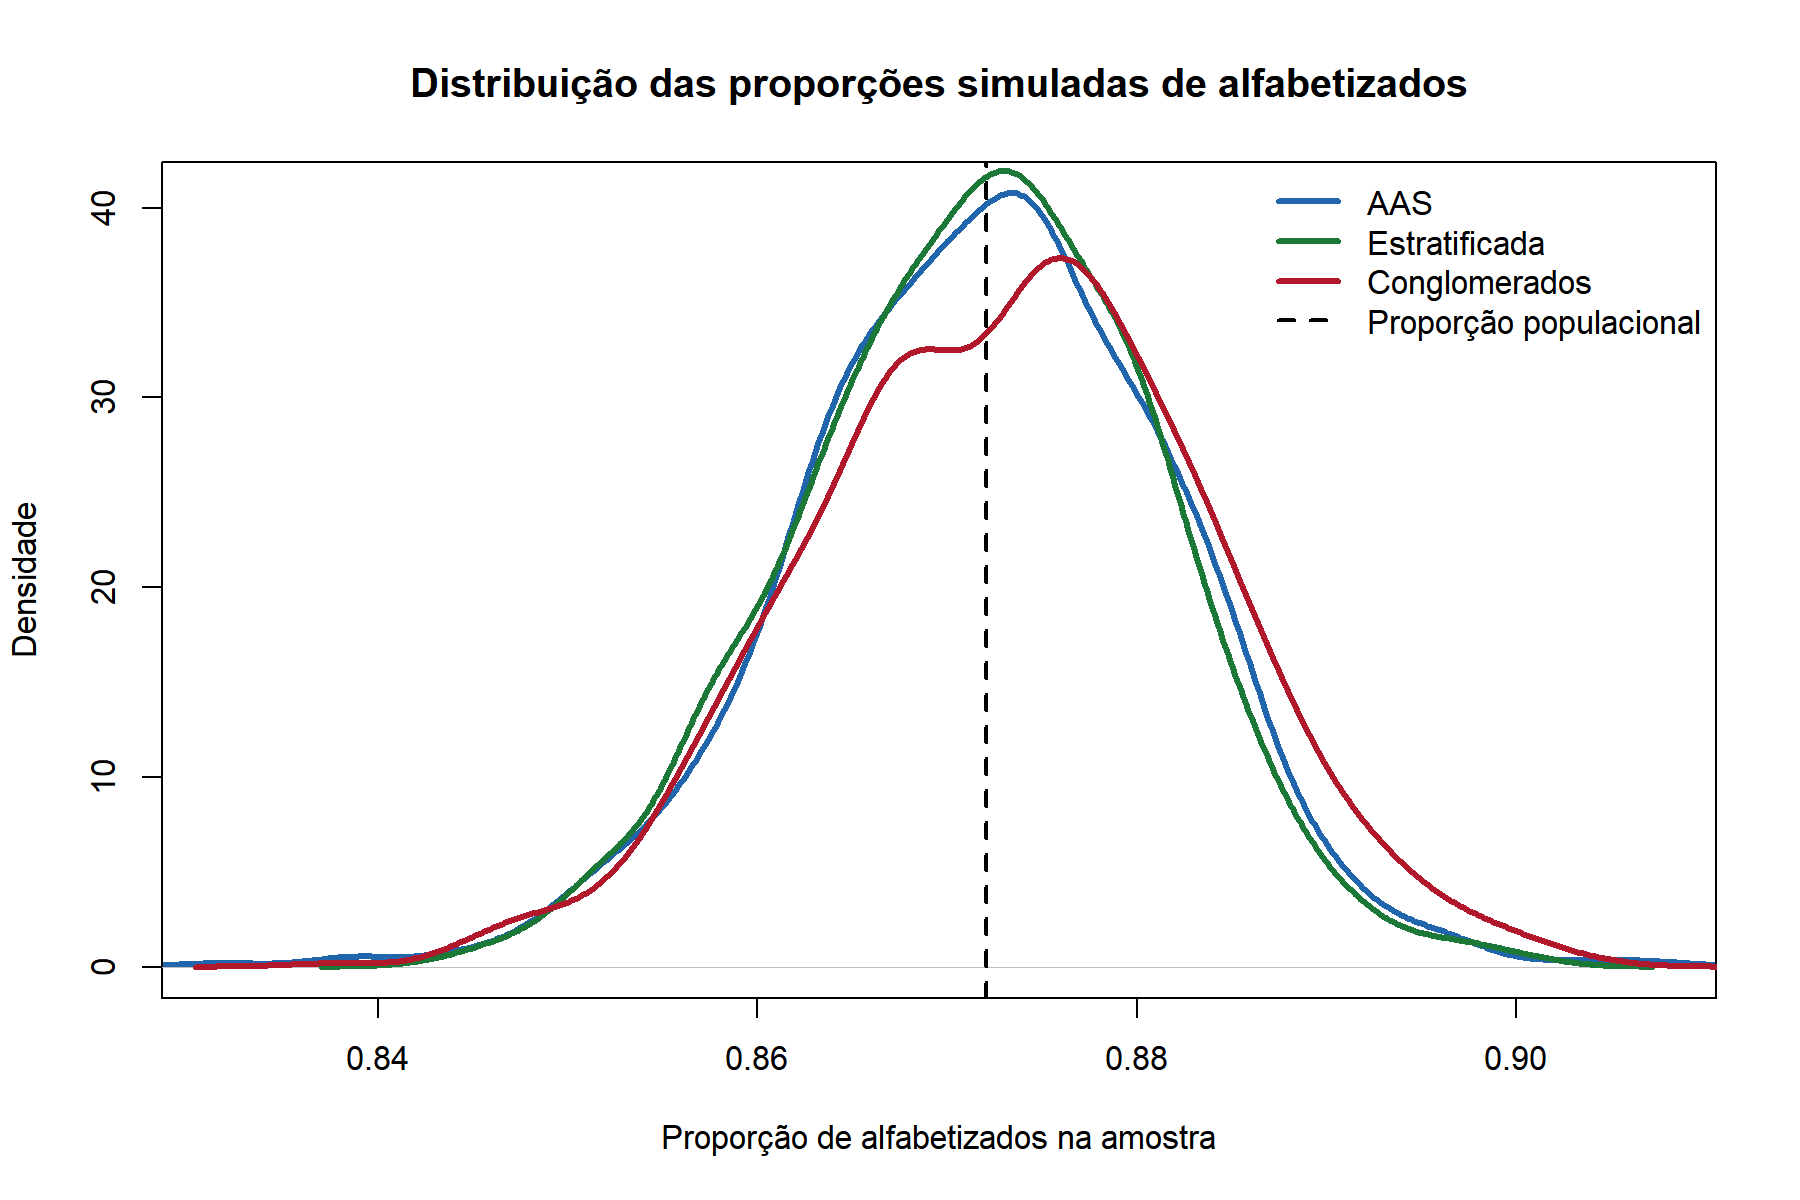
\includegraphics[width=0.92\textwidth]{grafico_distribuicoes.png}
\caption{Distribuição das proporções estimadas em 1.000 simulações para cada desenho amostral.}
\end{figure}

\section*{Interpretação}

O desenho estratificado produziu variância menor do que a AAS. O \textit{design effect} foi 0,909, ou seja, a variância da estimativa estratificada ficou cerca de 9,1\% abaixo da variância da AAS. Isso ocorre porque os estratos foram construídos a partir de uma característica associada à variável de interesse: a taxa média de alfabetização dos bairros. Quando os estratos são relativamente homogêneos por dentro e diferentes entre si, a estratificação reduz a oscilação das estimativas entre amostras.

O desenho por conglomerados produziu variância maior do que a AAS. O \textit{design effect} foi 1,149, indicando uma variância aproximadamente 14,9\% maior do que a variância da AAS. Esse resultado é esperado porque pessoas que vivem no mesmo setor censitário tendem a ser mais parecidas entre si do que pessoas sorteadas aleatoriamente em toda a cidade. Essa semelhança interna reduz a quantidade efetiva de informação trazida pela amostra.

Em termos práticos, a estratificação ajudou porque usou informação auxiliar relevante antes do sorteio. Já a amostragem por conglomerados aumenta a praticidade operacional, pois concentra entrevistas em setores sorteados, mas essa conveniência tem custo estatístico: a amostra fica menos dispersa geograficamente e, por isso, a variância tende a subir.

\section*{Conclusão}

Entre os três desenhos, a AAS funciona como referência simples e neutra. A estratificação foi o desenho mais eficiente para esta base, pois reduziu a variância mantendo o tamanho da amostra em 1.200 pessoas. O desenho por conglomerados foi menos eficiente estatisticamente, mas é justificável em situações reais de campo, nas quais visitar setores selecionados pode reduzir custo, tempo e logística de coleta.

\end{document}
